\documentclass{report}
\usepackage[utf8]{inputenc}
\usepackage[italian]{babel}
\usepackage[linktoc=all]{hyperref}
\usepackage{graphicx}
\usepackage{mathtools}
\usepackage{float}
\graphicspath{ {./images/} }
\hypersetup{
	colorlinks,
	citecolor=black,
	filecolor=black,
	linkcolor=black,
	urlcolor=black
}
\usepackage[a4paper,includeheadfoot,margin=2.54cm]{geometry}
\usepackage{fancyhdr}
\newcommand\hr{\par\vspace{-.5\ht\strutbox}\noindent\hrulefill\par}
\usepackage{enumitem}


\begin{document}
	
	\author{Davide Parpinello}
	\title{%
			\begin{Large}
				Appunti di\\
			\end{Large}
		Reti (F. Granelli)}
	\date{Aprile 2020}
	\maketitle
	
	\tableofcontents
	\renewcommand{\chaptermark}[1]{%
		\markboth{#1}{}}
	\addtocontents{toc}{\protect\hypertarget{toc}{}}
	\pagestyle{fancy}
	\fancyhf{}
	\rhead{\hyperlink{toc}{Reti}}
	\lhead{\leftmark}
	\rfoot{\thepage}
	
	\chapter{Roadmap}
	\section{Internet}
	
	Internet è costituito da milioni di dispositivi, chiamati \textbf{sistemi terminali}, collegati tra loro da collegamenti in rame, fibre ottiche, oppure via radio come onde elettromagnetiche o satelliti.
	\medskip\\
	La frequenza di trasmissione in internet è data dall'ampiezza di banda disponibile.
	\medskip\\Sulla rete internet inoltre sono presenti particolari host, denominati \textbf{router}, che si occupano di instradare i pacchetti verso la loro destinazione finale.
	\medskip\\Nello scambio di messaggi tra host vengono implementati dei \textbf{protocolli}, che ne definiscono formato e ordine d'invio, così come le azioni intraprese in fase di trasmissione e/o ricezione di un messaggio o un altro evento.
	\medskip\\Internet è un'infrastruttura di comunicazione per applicazione distribuita, viene anche chiamato "rete delle reti" ed è organizzato in modo gerarchico.
	\section{Ai confini della rete}
	Sul bordo della rete internet troviamo applicazioni e sistemi terminali, raggruppati tra loro e connessi tra di loro mediante collegamenti cablati e wireless.
	\medskip\\I sistemi terminali (o host) fanno girare diversi programmi applicativi e possono essere organizzati con architettura client/server oppure P2P.
	\medskip\\L'accesso a internet può avvenire mediante diversi modi:
	\begin{itemize}
		\item \textbf{Accesso residenziale:} viene utilizzato un modem dial-up o DSL.
		\item \textbf{Accesso aziendale:} una LAN collega i sistemi terminali di aziende e università all'\textbf{edge router}, i sistemi terminali sono collegati tra loro mediante uno switch ethernet.
		\item \textbf{Accesso wireless:} i terminali vengono collegati mediante \textbf{access point}.
		\item \textbf{Reti domestiche:} sono costituite da un modem DSL o via cavo, un router/firewall/NAT, switch ethernet e accesso wireless. Spesso queste funzioni vengono raggruppate in un unico dispositivo (modem/router).
	\end{itemize}
	\section{Il nucleo della rete}
	Al centro della rete si trovano invece router interconnessi tra loro, che creano quindi una rete delle reti.
	\medskip\\I dati nel nucleo della rete vengono trasferiti con due modalità differenti:
	\begin{itemize}
		\item \textbf{Commutazione di circuito:} è presente un circuito dedicato per l'intera durata della sessione
		\item \textbf{Commutazione di pacchetto:} i messaggi di una sessione utilizzano le risorse su richiesta, di conseguenza potrebbero dover attendere per accedere a un collegamento.
	\end{itemize}
	\subsection{Esempio di commutazione di circuito}
	Consideriamo un file L di 640.000 bit, un bitrate totale C da 1.536 Mbps, TDM con 24 slot/s, 500ms per stabilire la connessione.
	\medskip\\ Trovo inizialmente la capacità di un singolo slot:\[C_{1 slot} = \frac{C}{24} = 0.064 Mbps = 64 Kbps\]
	Successivamente calcolo il tempo necessario alla trasmissione:\[T_{tx} = \frac{L}{C_{1 slot}} = 10s\]
	Infine, calcolo il tempo totale:\[T_{tot}=500ms+10s=10,5s\]
	\subsection{Esempio di commutazione di circuito}
	I secondi necessari per trasmettere un pacchetto in uscita su un collegamento da R bps sono dati da L/R, mentre il ritardo 3L/R
	\subsection{Confronto fra commutazione di pacchetto e di circuito}
	La commutazione di pacchetto consente un utilizzo della rete da parte di maggiori utenti, ed è ottima per i dati a raffica.\medskip\\ Dal lato negativo, presenta un'eccessiva congestione, causando ritardi e perdite di pacchetti. Sono quindi necessari protocolli per il trasferimento affidabile e per il controllo della congestione.
	\subsection{Struttura gerarchica}
	La rete internet ha una struttura fondamentalmente gerarchica:
	\begin{itemize}
		\item Al centro sono presenti \textbf{ISP di livello 1}, che offrono una copertura nazionale e/o internazionale
		\begin{itemize}
			\item Comunicano tra loro come fossero pari
		\end{itemize}
		\item \textbf{ISP di livello 2:} ISP più piccoli, copertura nazionale/distrettuale.
		\begin{itemize}
			\item Si può connettere solo ad alcuni ISP di livello 1 e ad altri di livello 2
			\item Paga l'ISP di livello 1 che gli fornisce la connettività per il resto della rete
		\end{itemize}
		\item \textbf{ISP di livello 3 e ISP locali (di accesso):}
		\begin{itemize} 
			\item sono le reti "ultimo salto", le più vicine agli host
			\item Sono clienti degli ISP di livello superiore che li collegano all'intera internet.
		\end{itemize}
	\end{itemize}
	Un pacchetto attraversa un sacco di reti, dal livello più basso fino al principale e poi nuovamente a scendere.
	\section{Ritardi, perdite e throughput nelle reti a comunicazione di pacchetto}
	Nella rete si verificano dei ritardi quando il tasso di arrivo dei pacchetti eccede la capacità di evaderli, con la conseguenza che vengono accodati nei buffer del router in attesa del proprio turno. Se non ci sono buffer liberi i pacchetti vengono scartati e ritrasmetti dal nodo precedente o, in alcuni casi, non venire proprio ritrasmessi.
	\medskip\\ Quattro cause di ritardo dei pacchetti sono le seguenti:
	\begin{enumerate}
		\item Ritardo di elaborazione sul nodo
		\begin{itemize}
			\item Controllo errori sui bit
			\item Determinazione del canale di uscita
		\end{itemize}
		\item Ritardo di accodamento
		\begin{itemize}
			\item Attesa di trasmissione
			\item Livello di congestione del router
		\end{itemize}
		\item Ritardo di trasmissione (L/R)
		\begin{itemize}
			\item R = frequenza di trasmissione del collegamento
			\item L = lunghezza del pacchetto
		\end{itemize}
		\item Ritardo di propagazione (d/s)
		\begin{itemize}
			\item d = lunghezza dl collegamento fisico 
			\item s = velocità di propagazione del collegamento (\textasciitilde} \(2 \cdot 10^8\) m/s)
		\end{itemize}
	\end{enumerate}
	\begin{center}
		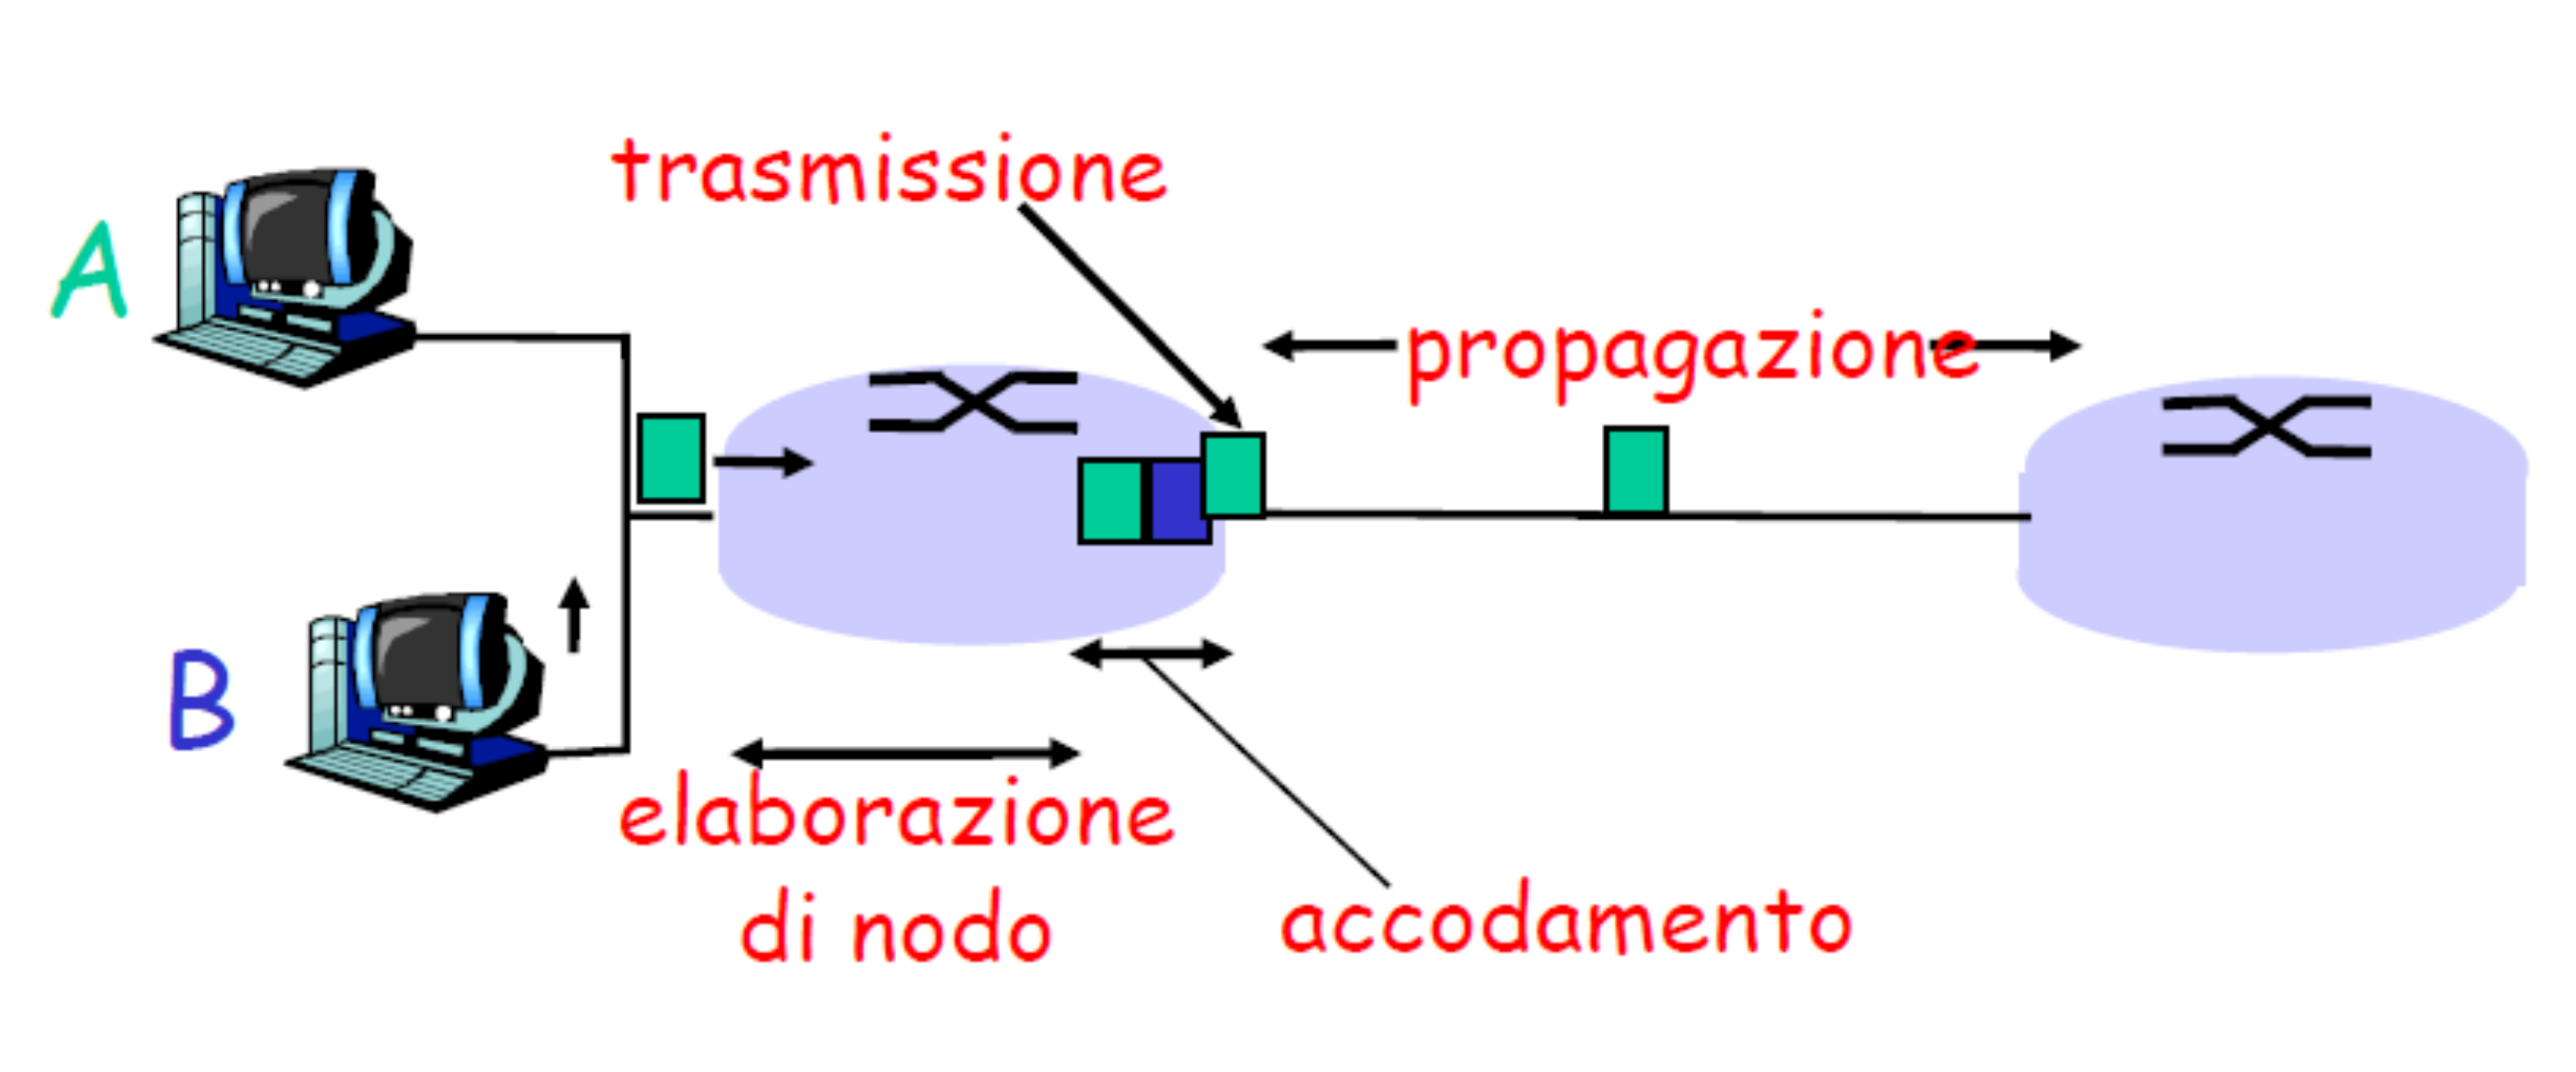
\includegraphics[width=0.7\linewidth]{ritardi.png}
	\end{center}
	\subsection{Ritardo di un nodo}
	Il ritardo di un nodo è dato dalla seguente formula:
	\begin{equation}
		d_{nodal} = d_{proc}+d_{queue}+d_{trans}+d_{prop}
	\end{equation}
	dove:
	
	
\end{document}